\documentclass[hyperref={pdfpagelabels=false}]{beamer}
\setbeamercolor{background canvas}{bg=white}
\usepackage{graphicx,lmodern,subfigure,ulem,color,graphicx,tikz,booktabs,natbib}
\usepackage{mathrsfs}
\usetheme{Warsaw}
%\definecolor{beamer@blendedblue}{rgb}{0.1,0.5,0.1}
%\definecolor{ForestGreen}{RGB}{60, 140, 60}
%\setbeamercolor{structure}{fg=beamer@blendedblue}
\setbeamertemplate{navigation symbols}{}
\setbeamertemplate{footline}[frame number]
\bibliographystyle{chicago}
\newcommand{\spitem}{\vspace{.3cm}\item}
\newcommand{\elas}{$E_{labor}$}
%\def \FigPath {Users\th3\Documents\Job_Market_Paper\Code\Figures} 
\DeclareMathOperator{\E}{\mathbb{E}}



\title{Uncertainty Shocks and Financial Shocks}
\author{Marco Brianti}
\institute{Boston College}
\date{October 2018}

\usetheme[
outer/progressbar=foot,
outer/numbering=none
]{metropolis}


\begin{document}
	
	\frame{\titlepage \begin{center} Dissertation Project \end{center} }
	





\frame{\frametitle{Financial Shocks and Uncertainty Shocks}
	
	Stock and Watson (2012); Caldara et al. (2016) among others shown that uncertainty shocks and financial shocks are deeply confounded.
	
	
	\
	
	
	$$
	corr(\iota^{EBP}_t,\iota^{JLN}_t) \approx 0.45
	$$
	
	
	\
	
	
	where $\iota^{EBP}_t$ is an unpredictable innovation in the \textbf{excess bond premium} from Gilchrist and Zakrajzek (2012) and $\iota^{JLN}_t$ is an unpredictable innovation in the \textbf{uncertainty proxy} from Jurado et al. (2015).
	

	

	
	
	
}

\frame{\frametitle{Both a theoretical and empirical question}

	Literature did not succeed yet to disentangle the two exogenous sources for two main reasons:
\begin{enumerate}
	\item Simultaneity
	\begin{itemize}
		\item Both types of variables are fast moving
				\end{itemize}	
			\item Effect on observables
			
			\begin{itemize}
			\item They have the same qualitative effects on prices and quantities
\end{itemize}
\end{enumerate}

\

\

As a result, both \textbf{zero-impact restrictions} cannot be used and \textbf{internal instruments} are not available.
	
}

\frame{\frametitle{This Project}
	
	I want to take a step back and argue that it is conceptually wrong to disentangle these two shocks as defined by the literature.
	
	\
	
	
	From a theoretical point of view, uncertainty shocks can potentially be a primitive source of financial shocks.
	
	\
	
	
	It is more important to gauge how much of the combinations of these shocks appears to be
	\begin{itemize}
		\item a credit supply shock $\Rightarrow$ \textbf{financial shock}
		\item a credit demand shock $\Rightarrow$ \textbf{macro uncertainty shock}
	\end{itemize}
	
	
}
	


\frame{\frametitle{Main Contribution}
	
	
	\begin{enumerate}
		
		\item I present evidence and theory of an \textbf{internal instrument} able to disentangle shifts in credit supply and demand. 


\

\

\


		
		\item I provide a \textbf{new econometric method} which can be applied to disentangle two structural shocks when an internal instrument is available.
		
	\end{enumerate}
	

}

\frame{\frametitle{Corporate Cash Reserves}
	
\textbf{Cash reserves} (or \textbf{cash holdings}) refer to money or extremely liquid short-term investment which an individual corporation saves in order to be ready to cover any emergency funding or short-term requirements. 

\

The typical U.S. large firm has cash equal to about 10\% and 15\% of total assets.

\

Together with current cash flow is consider the most important \textbf{internal source of finance}.
}


\frame{\frametitle{Cash Reserves and Financial Frictions}
	
	

		
Almeida, Campello, Weisbach, 2004. \textit{The Journal of Finance} 	
		\begin{itemize}
			\item[$\Rightarrow$] Financially constrained firms tend to build larger cash reserves as a buffer against potential credit supply shocks.
		\end{itemize}
		
		
		\
		
Kaplan and Zingales, 1997. \textit{Quarterly Journal of Economics}
		\begin{itemize}
	\item[$\Rightarrow$] Investment is positive related to cash reserves when firms are financially constrained.
\end{itemize}
		
		\
		
		Campello, Graham, Harvey, 2010. \textit{Journal of Financial Economics}
				\begin{itemize}
			\item[$\Rightarrow$] After the 2008-09 credit supply shock, cash reserves decrease because adopted as internal source of finance. 
		\end{itemize}
		
	
}

		\frame{\frametitle{Cash Reserves and Uncertainty}
	
Bloom, Mizen, Smietanka (2018). \textit{Working Paper}
	\begin{itemize}
		\item[$\Rightarrow$] Higher economic uncertainty in the years 2007-09 is related to an increase in cash holdings.
			\end{itemize}


	\
	
	\
	
Alfaro, Bloom, Lin (2018). \textit{NBER Working Paper}
	
	\begin{enumerate}
		\item[$\Rightarrow$] Firms accumulate cash reserves and short-term liquid instruments following uncertainty rises.
	\end{enumerate}
	

	

	
}
	
	
	\frame{\frametitle{Economic Intuition I}	
		
To provide an economic intuition of the differential response of \textbf{cash holdings} to uncertainty and financial shocks, I present a properly augmented model in the spirit of 
\begin{itemize}
	\item Almeida, Campello, and Weisbach (2004)
	\item Han and Qiu (2007)
\end{itemize}


\

It is a simple representation of a dynamic setting where a credit-constrained profit-maximizing firm has a trade-off between present and future investment opportunities


		
	}

\frame{\frametitle{Model}

\begin{itemize}
	\item[]
\begin{itemize}
     \item[Period 0] $ \ \ \ d_0 = y_0 + b_0 - i_0 - c$
	
	\
	
	
	\item[Period 1] $ \ \ \ d_1 = y_1 + b_1 - i_1 + c, \ \ \ $ where $ \ y_1 \sim F$
	
	\
	
	
	\item[Period 2] $ \ \ \ d_2 = g(I_0) - b_0 + h(I_1) - b_1$
\end{itemize}
\end{itemize}

\begin{eqnarray*}
	\begin{aligned}
\max_{\{ b_t,i_t,c \}_{t=0,1}} \ \ &\E \Big[  d_0 + d_1 + d_2     \Big| F  \Big] \\
\text{subject to} \ \ &b_t \leq (1 - \tau_t)i_t, \ \ \ t = 0,1 \\
&d_t \geq 0, \ \ \ t = 0,1,2
\end{aligned}
\end{eqnarray*}
	
}
	
	

\frame{\frametitle{Solution}
	
	Financially constrained firm: $I^*_t < I^{FB}_t$ for $t=0,1$
\begin{itemize}
	\item[$\Rightarrow$] $b_t = (1 - \tau_t)i_t \ \ $ for $ \ t=0,1$
	\item[$\Rightarrow$] $d_t = 0 \ \ $ for $ \ t=0,1$
\end{itemize}
which implies $I_0 = \frac{y_0 - c}{\tau_0}$ and $I_1 = \frac{y_1 + c}{\tau_1}$. Objective function is,
\begin{eqnarray*}
	\max_c g \bigg( \frac{y_0 - c}{\tau_0 } \bigg) - \frac{y_0 - c}{\tau_0 } +   \E \bigg[  h \bigg( \frac{y_1 + c}{\tau_1 } \bigg) - \frac{y_1 + c}{\tau_1 }   \bigg| F     \bigg]
	\end{eqnarray*}
and optimal condition for $c^*(\tau_0,F)$ is
\begin{eqnarray*}
\underbrace{g' \bigg( \frac{y_0 - c^*(\tau_0,F)}{\tau_0 } \bigg)}_{\text{Marginal Return of $I_0$}} = \underbrace{\E \bigg[  h' \bigg( \frac{y_1 + c^*(\tau_0,F)}{\tau_1 } \bigg)  \bigg| F  \bigg]}_{\text{$\E$ Marginal Return of $I_1$}}
\end{eqnarray*}

}

\frame{\frametitle{Comparative Statics}
	Given the Euler equation for cash $c$,
	\begin{eqnarray*}
		\underbrace{g' \bigg( \frac{y_0 - c^*(\tau_0,F)}{\tau_0 } \bigg)}_{\text{Marginal Return of $I_0$}} = \underbrace{\E \bigg[  h' \bigg( \frac{y_1 + c^*(\tau_0,F)}{\tau_1 } \bigg)  \bigg| F  \bigg]}_{\text{$\E$ Marginal Return of $I_1$}}
	\end{eqnarray*}

\
	
\textbf{Uncertainty shock}: $y_1 \sim Q$ which is mean-preserving spread in $F$
	\begin{enumerate}
	\item[$\Rightarrow$] $c^*(\tau_0,Q) > c^*(\tau_0,F)$ as long as $h'''(\cdot) > 0$
\end{enumerate}

\

\textbf{Financial shock}: $\tau_0^f > \tau_0$ which is a decrease in $b_0$
	\begin{enumerate}
	\item[$\Rightarrow$] $c^*(\tau_0^f,Q) < c^*(\tau_0,F)$ 
\end{enumerate}

}



\frame{\frametitle{Penalty Functions (I)}

Penalty functions is a maximization problem where the importance of the constraint depends on some assumptions.

\

Consider the standard constrained maximization problem,
$$
\max_x f(x) \ \ \text{s.t} \ \ g(x) \geq 0
$$
a penalty function is an unconstrained maximization problem
$$
\max_x f(x) + G \big( g(x) \big) 
$$


$\Rightarrow$ Assumptions on $G(\cdot)$ determines the importance of $g(x)$.


}


\frame{\frametitle{Penalty Functions (II)}
	
Given $\max_x f(x) \ \ \text{s.t} \ \ g(x) \geq 0$, I assume $G(\cdot)$ to be linear,
$$
\max_x f(x) + \delta  g(x), \ \ \ \delta > 0
$$
$\Rightarrow$ the larger $\delta$, the more important $g(x)$

\

Applied to SVARs, PFA has the flavor of \textbf{sign restrictions} but with the advantage that the problem is \textbf{just identified}. 

\

\textbf{Shortcoming}: parameter $\delta$ is exogenously chosen making the identification strategy less credible.
	
	
}



\frame{\frametitle{Identification (I)}
	
	Given the reduced-form system $X_t = \textcolor{red}{B} X_{t-1} + \iota_t$ where 
	\begin{itemize}
		\item $X_t = [U_t \ \ F_t \ \ Y_t]'$ where $Y_t$ are macroeconomic variables.
		\item $\iota_t' \iota_t = \Sigma_{\iota}$
	\end{itemize}
	\textbf{Step 1}
	\begin{eqnarray*}
		\max_{\gamma_{U}} \ & \ \sum_{t=0}^K e'_U B^t \tilde{A}_0 \gamma_U + \delta e'_{C} \tilde{A}_0 \gamma_U \\
		\text{subject to} \ & \ \delta \geq 0 \ \ \text{and} \ \ \gamma_U \gamma_U' = 1
	\end{eqnarray*}
	\textbf{Step 2}
	\begin{eqnarray*}
		\max_{\gamma_{F}} \ & \ \sum_{t=0}^J e'_F B^t \tilde{A}_0 \gamma_F - \delta e'_{C} \tilde{A}_0 \gamma_F \\
		\text{subject to} \ & \ \delta \geq 0, \ \ \gamma_F \gamma_F' = 1 \ \ \text{and} \ \ \gamma_U \gamma_F' = 0
	\end{eqnarray*}
	where $\tilde{A}_0 \tilde{A}'_0 = \Sigma_{\iota}$ and $e_j$ is a selection vector of variable $j$.
	
}


\frame{\frametitle{Identification (I)}
	
	Given the reduced-form system $X_t = B X_{t-1} + \iota_t$ where 
	\begin{itemize}
		\item $X_t = [U_t \ \ F_t \ \ C_t \ \ Y_t]'$ 
		\item $\iota_t' \iota_t = \Sigma_{\iota}$
	\end{itemize}
	\textcolor{red}{\textbf{Step 1 - Uncertainty Shock}}
	\begin{eqnarray*}
		\max_{\gamma_{U}} \ & \ \sum_{t=0}^K e'_U B^t \tilde{A}_0 \gamma_U + \delta e'_{C} \tilde{A}_0 \gamma_U \\
		\text{subject to} \ & \ \delta \geq 0 \ \ \text{and} \ \ \gamma_U \gamma_U' = 1
	\end{eqnarray*}


An uncertainty shock maximizes its effect on uncertainty over the first $K$ quarters with penalty (merit) $\delta$ if cash is negative (positive) on impact.
	
}

\frame{\frametitle{Identification (I)}

Given the reduced-form system $X_t = B X_{t-1} + \iota_t$ where 
\begin{itemize}
\item $X_t = [U_t \ \ F_t \ \ Y_t]'$ where $Y_t$ are macroeconomic variables.
\item $\iota_t' \iota_t = \Sigma_{\iota}$
\end{itemize}
\textcolor{red}{\textbf{Step 2 - Financial Shock}}
\begin{eqnarray*}
	\max_{\gamma_{F}} \ & \ \sum_{t=0}^J e'_F B^t \tilde{A}_0 \gamma_F - \delta e'_{C} \tilde{A}_0 \gamma_F \\
	\text{subject to} \ & \ \delta \geq 0, \ \ \gamma_F \gamma_F' = 1 \ \ \text{and} \ \ \gamma_U \gamma_F' = 0
\end{eqnarray*}
A financial shock maximizes its effect on credit spread over the first $J$ quarters with penalty (merit) $\delta$ if cash is positive (negative) on impact.
	
}





\frame{\frametitle{Identification (I)}
	
	Given the reduced-form system $X_t = B X_{t-1} + \iota_t$ where 
	\begin{itemize}
		\item $X_t = [U_t \ \ F_t \ \ Y_t]'$ where $Y_t$ are macroeconomic variables.
		\item $\iota_t' \iota_t = \Sigma_{\iota}$
	\end{itemize}
	\textbf{Step 1 - Uncertainty Shock}
	\begin{eqnarray*}
		\max_{\gamma_{U}} \ & \ \sum_{t=0}^K e'_U B^t \tilde{A}_0 \gamma_U + \textcolor{red}{\delta} e'_{C} \tilde{A}_0 \gamma_U \\
		\text{subject to} \ & \ \delta \geq 0 \ \ \text{and} \ \ \gamma_U \gamma_U' = 1
	\end{eqnarray*}
	\textbf{Step 2 - Financial Shock}
	\begin{eqnarray*}
		\max_{\gamma_{F}} \ & \ \sum_{t=0}^J e'_F B^t \tilde{A}_0 \gamma_F - \textcolor{red}{\delta} e'_{C} \tilde{A}_0 \gamma_F \\
		\text{subject to} \ & \ \delta \geq 0, \ \ \gamma_F \gamma_F' = 1 \ \ \text{and} \ \ \textcolor{red}{\gamma_U \gamma_F' = 0}
	\end{eqnarray*}
	where $\tilde{A}_0 \tilde{A}'_0 = \Sigma_{\iota}$ and $e_j$ is a selection vector of variable $j$.
	
}

\frame{\frametitle{Identification (II)}

I suggest a \textbf{general approach} where $\delta$ is treated as an endogenous parameter chosen by the data.
\begin{itemize}
\item[$\Rightarrow$] Given the problem above, set $\delta$ such that $\gamma_U \gamma'_F = 0$
\end{itemize}

\begin{center}
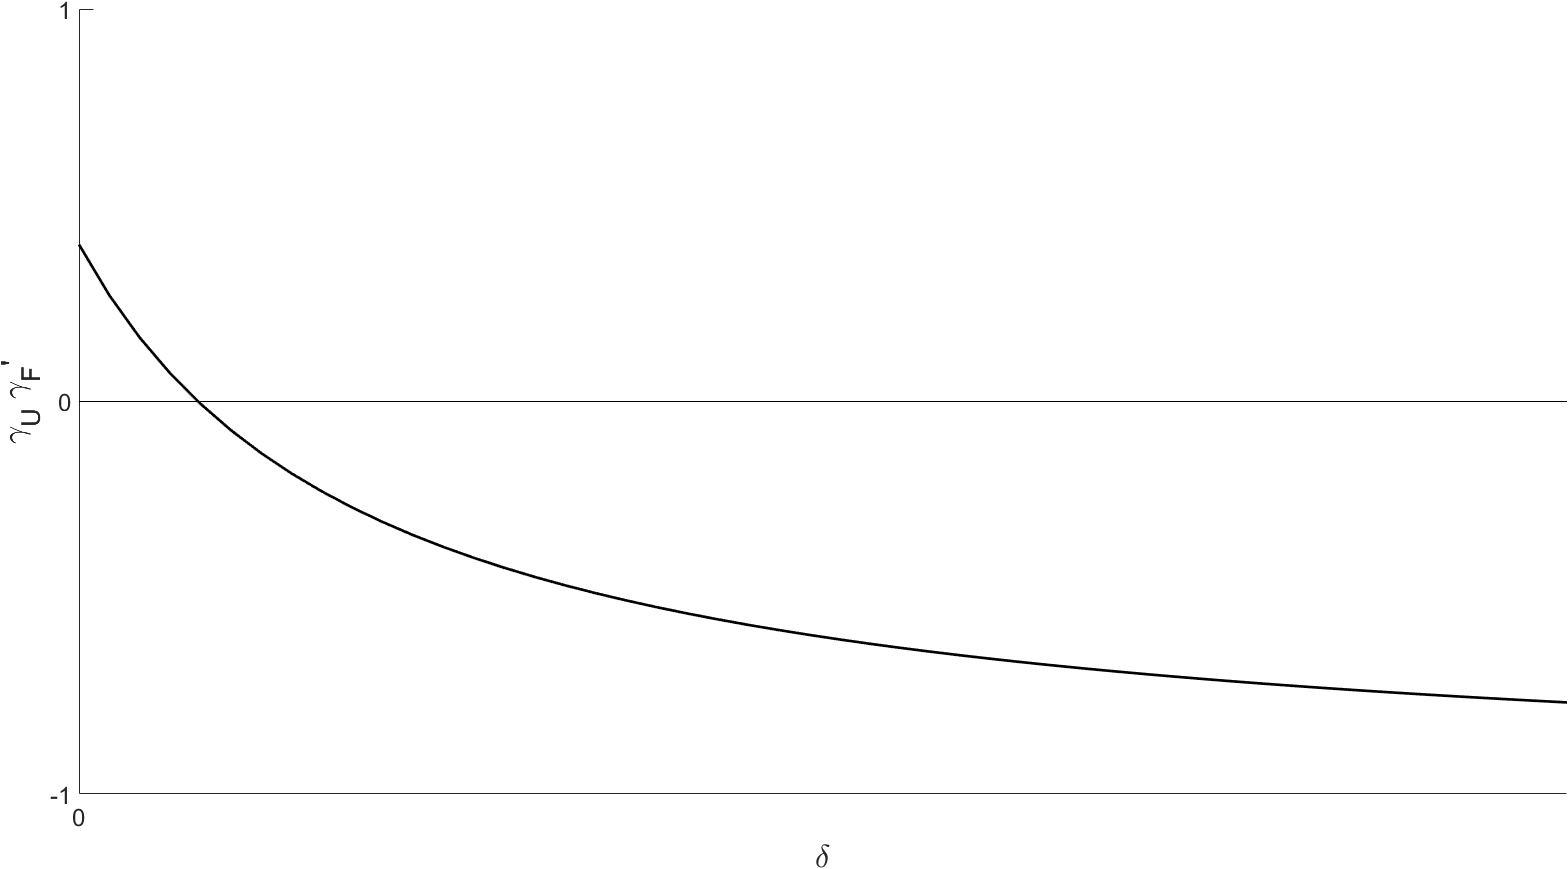
\includegraphics[scale=0.15]{fig_GPFA_intuition_figure_}
\end{center}

\textbf{Intuition.} Internal instrument intervention should be strong enough such that $\gamma_U \gamma_F' = 0$.






}

\frame{\frametitle{Results - Uncertainty Shock}

\begin{center}
	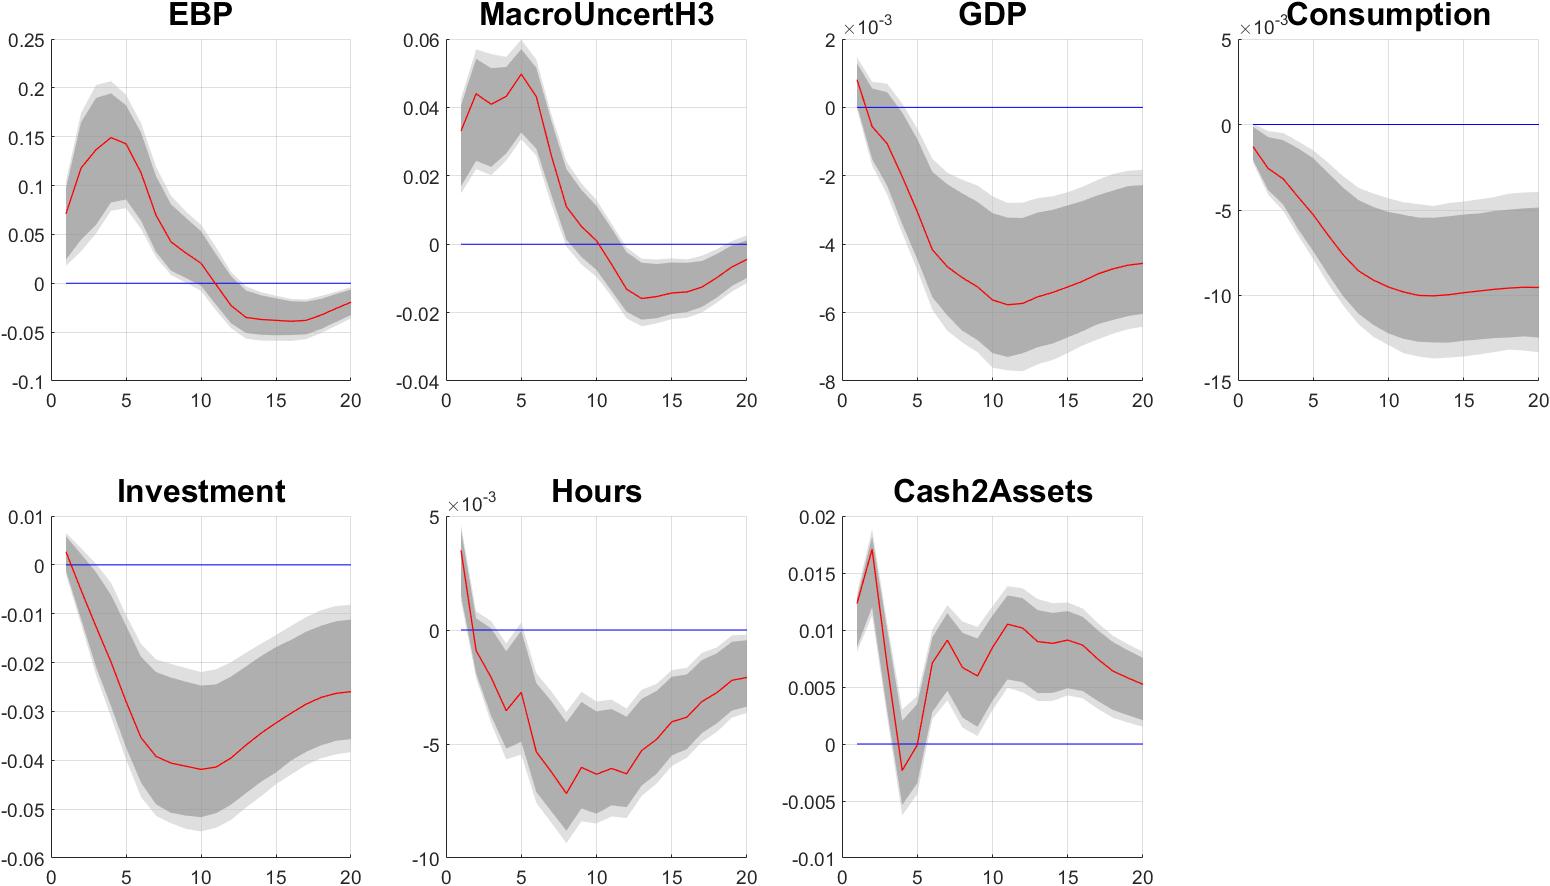
\includegraphics[scale=0.27]{fig_Uncertainty_Shock_GPFA_Compustat_3lags_03-Oct-2018_12_25_58}
\end{center}	

	
}

\frame{\frametitle{Results - Financial Shock}
	
	\begin{center}
		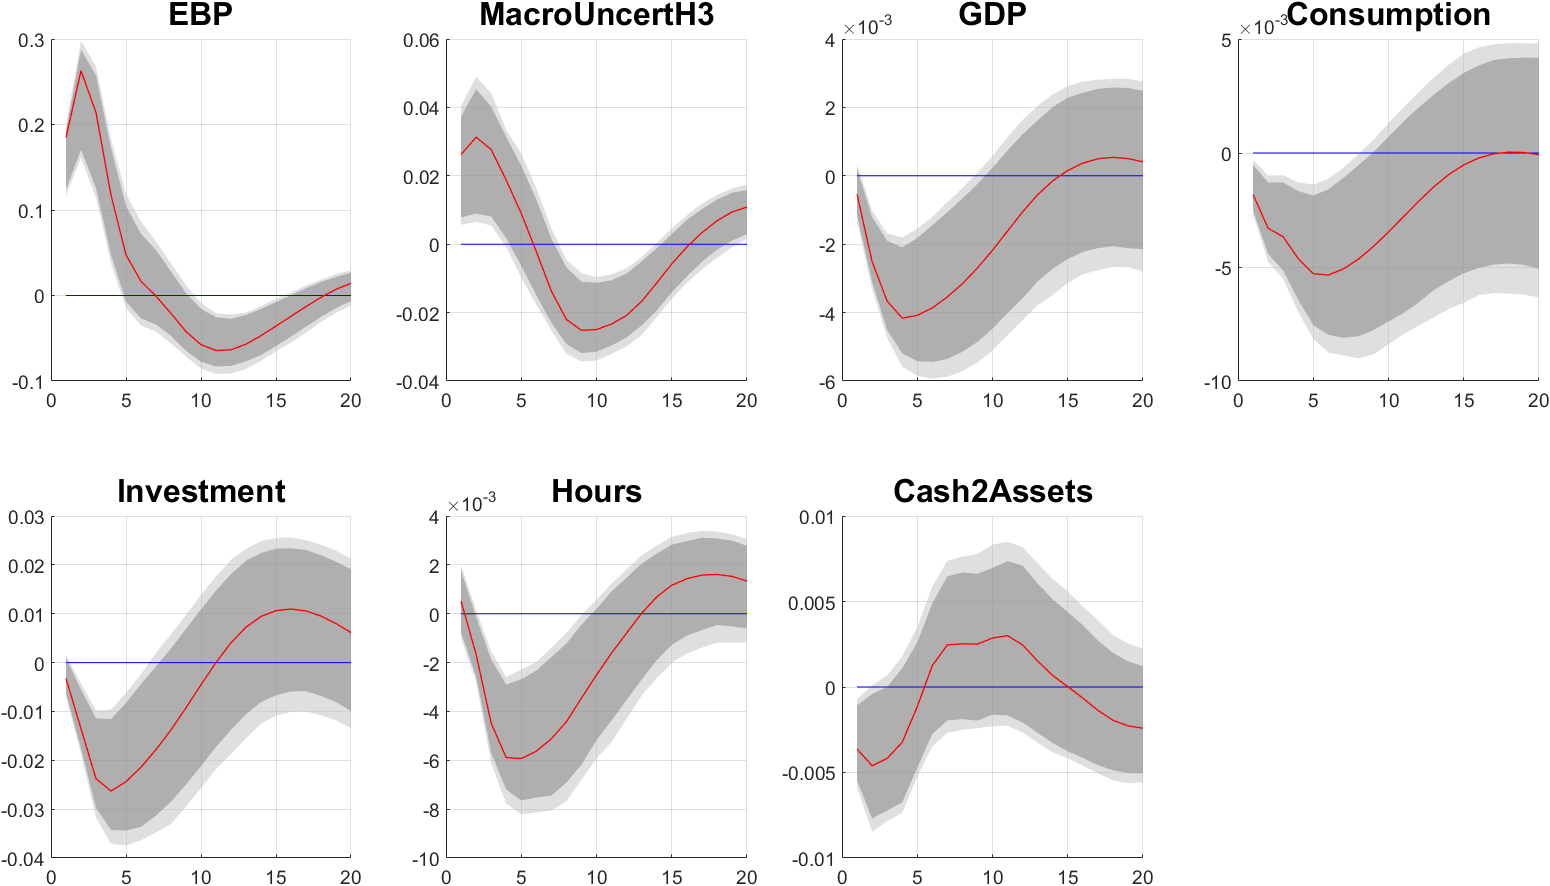
\includegraphics[scale=0.27]{fig_Financial_Shock_GPFA_Compustat_3lags_03-Oct-2018_12_26_00}
	\end{center}	
		
}



\frame{\frametitle{Results - Variance Explained}
	
	\begin{center}
		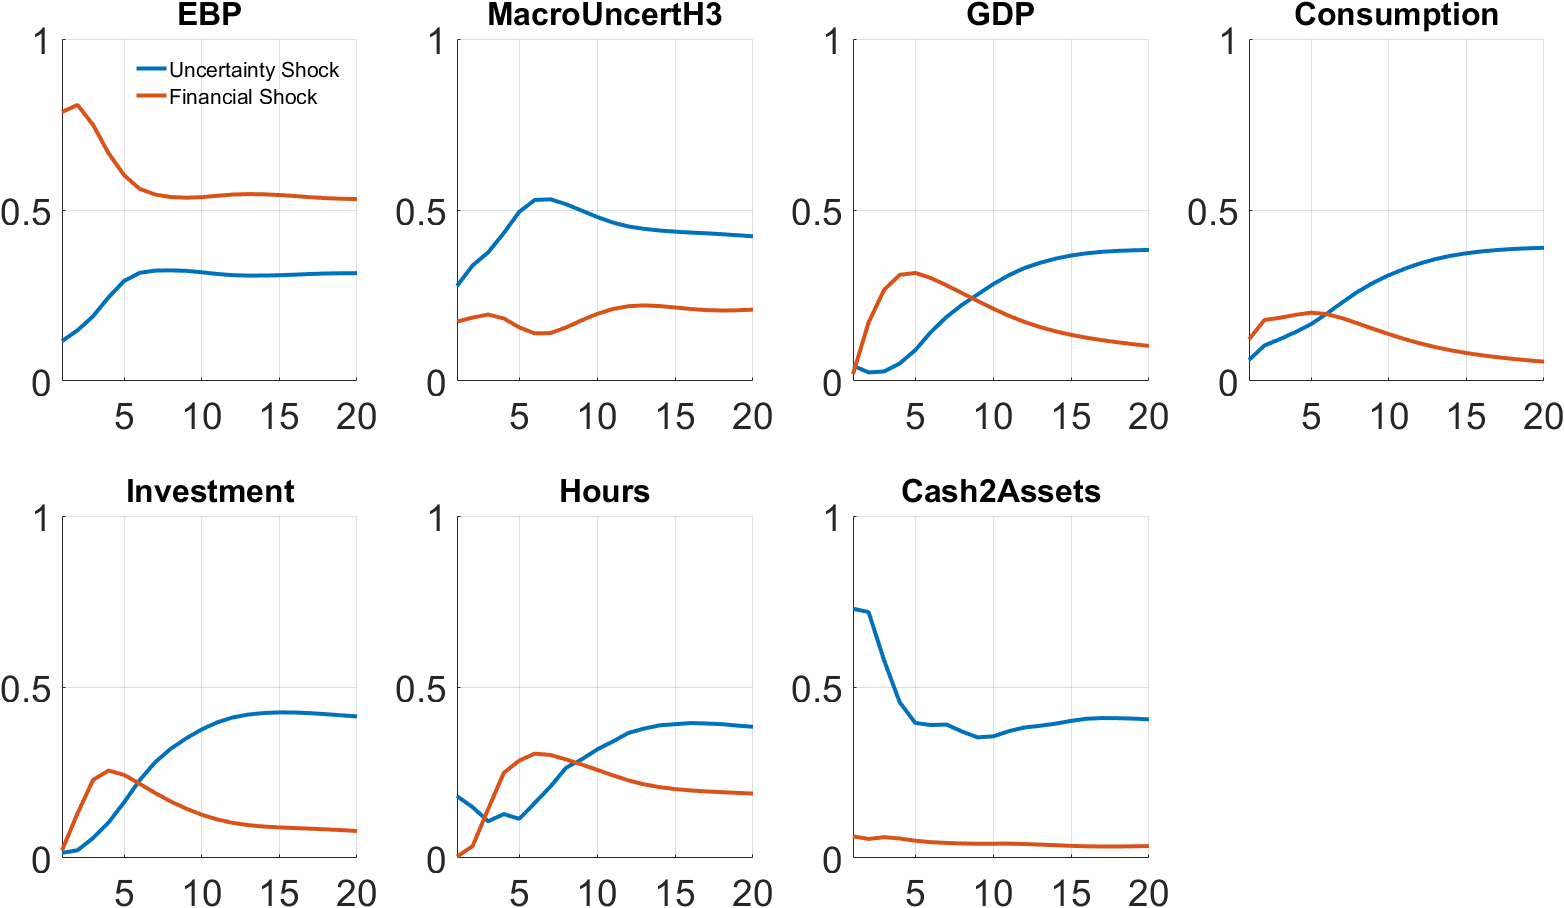
\includegraphics[scale=0.27]{fig_var_dec_vardec_GPFA_Compustat_3lags_03-Oct-2018_12_37_32}
	\end{center}	
	
}

















\end{document}